\documentclass[article]{elsarticle}

\usepackage{lineno,hyperref}
\modulolinenumbers[5]

\journal{Journal of \LaTeX\ Templates}

%%%%%%%%%%%%%%%%%%%%%%%
%% Elsevier bibliography styles
%%%%%%%%%%%%%%%%%%%%%%%
%% To change the style, put a % in front of the second line of the current style and
%% remove the % from the second line of the style you would like to use.
%%%%%%%%%%%%%%%%%%%%%%%

%% Numbered
%\bibliographystyle{model1-num-names}

%% Numbered without titles
%\bibliographystyle{model1a-num-names}

%% Harvard
%\bibliographystyle{model2-names.bst}\biboptions{authoryear}

%% Vancouver numbered
%\usepackage{numcompress}\bibliographystyle{model3-num-names}

%% Vancouver name/year
%\usepackage{numcompress}\bibliographystyle{model4-names}\biboptions{authoryear}

%% APA style
%\bibliographystyle{model5-names}\biboptions{authoryear}

%% AMA style
%\usepackage{numcompress}\bibliographystyle{model6-num-names}

%% `Elsevier LaTeX' style
\bibliographystyle{elsarticle-num}
%%%%%%%%%%%%%%%%%%%%%%%

\begin{document}

\begin{frontmatter}

\title{Open Power System Data - Frictionless data for modelling}
\iffalse
%% Group authors per affiliation:
\author{Elsevier\fnref{myfootnote}}
\address{Radarweg 29, Amsterdam}
\fntext[myfootnote]{Since 1880.}


%% or include affiliations in footnotes:
\author[mymainaddress,mysecondaryaddress]{Elsevier Inc}
\ead[url]{www.elsevier.com}

\author[mysecondaryaddress]{Global Customer Service\corref{mycorrespondingauthor}}
\cortext[mycorrespondingauthor]{Corresponding author}
\ead{support@elsevier.com}

\address[mymainaddress]{1600 John F Kennedy Boulevard, Philadelphia}
\address[mysecondaryaddress]{360 Park Avenue South, New York}
\fi
\begin{abstract}
\begin{itemize}
    \item Power System Modelling is heavily depending on high quality data
    \item Transparency of it highly depends on the question if input data is provided
    \item Main challenges are to (i) use just openly available data, (ii) to preprocess the data in a transparent way (iii) to verify the data
     \item This article presents an approach to tackle these challenges
    %\item This article presents an approach to tackle these challenges, summarizes remaining legal issues and concludes suggestions on the requirements to progress on energy data provision
\end{itemize}
\end{abstract}

\begin{keyword}
\sep \sep 
\end{keyword}

\end{frontmatter}

\linenumbers

\section*{NOTES}
\begin{itemize}
    \item Irgendwo noch Legal Status, zumindest kurz erwaehnen: Legal Context: MIT for the scripts, but licensing the data itselfs is facing some problems, explain the lawyer assessments and communication with the original data owners
    \item Geographical Coverage: Für alle 5 data packages die Karte aus der Präsentation vom Abschlussworkshop integrieren, ja Unterpunkt oder in der Übersicht??
\end{itemize}

\section{Introduction (Frauke)}
\label{Introduction}

\subsection{Need for quantitative power sector modelling}
Energy research as well as policy advice are based on quantitative computer models. The number of models, especially power sector models has increased significantly within the last years. With a rising amount of fluctuating renewable wind and solar power, temporal resolution has become increasingly important since only then flexibility of power plants can be taken into account. Studies based on power sector models include price i.a. forecasts, interplay of wind and solar, ramping requirements for thermal power plants, storage requirements or optimal configurations of 100\% renewable power sectors and their respective transition pathways.

\subsection{Extensive input data requirements}
The optimisation or simulations performed with these power plant models heavily depend on various input data. Since most investigations start from the conditions of the power sector today, generation capacities as well as time series of load, prices as well as wind and solar power generation are particularly relevant. Additional data requirements also include inter-connector capacities, fuel prices, hydro reservoir inflows, district heating demand or system service requirements or potentials for renewable sources. However, the intersection of data required for all power sector models are existing capacities as well as load time series and renewable power feed-in.

\subsection{Availability of data}
A lot of data is available - but dispersed, poorly documented and ill-formatted

Although energy data availability has grown over the last years, data search, processing and validation still constitutes a significant share of the work load of power system modelling. This is due to
\begin{itemize}
    \item the required combination of several different sources
    \item difficult discoverability
    \item manual download of different files
    \item merging of different file-formats and formatting
    \item lack of a standardised nomenclature and classification of energy technologies and sources
    \item poorly documented original data, e.g. lack of meta data
    \item quality of input data which require a verification process (e.g inconsistencies, obvious errors, gaps in data)
\end{itemize}

Additionally, many of they openly available data is subject to unclear or restrictive terms of use. Actually, confusion around copyright is one of the main challenges for data sharing \url{https://figshare.com/articles/Whitepaper_Practical_challenges_for_researchers_in_data_sharing/5975011}

Concluding, data processing, maintenance and verification is a major obstacle and work load for power system modellers. Since it is performed by different teams in parallel isolation, efficiency could significantly improve if done in collaboration. Also the quality of the processed data could significantly improve by knowledge sharing of the large amount of power system data users. The project \textit{Open Power System Data (OPSD)} aims at harvesting the efficiency and quality gain for the power modelling community by collecting, checking, processing, aggregating, documenting and publishing data required for power modelling on an online platform. 

The concept and methods of \textit{Open Power System Data} is described in section \re
{sec:OPSD}, while section \ref{sec:packages} explains the approach and content of the resulting five data packages. Finally, we reflect on the current usage of the data packages as well as possible extensions \ref{sec:discussion}.    f
\section{OPSD: frictionless data for modelling (Ingmar)}
\label{OPSD}
\subsection{General idea}
gather "official" data in one place, foramt it nicely, quality checks / improvements; concept of data packages 

\subsection{IT concept}
"leightweight", open software, GitHub etc., data packages, scripts including documentation, storage of original data sources, version-control, metadata (json)

\subsection{Data standards}
Frictionless data (OKF), evtl.in 2.3 mit reinziehen)

\subsection{Some (careful) data modifications}
wenn möglich und sinnvoll, hier high-level Beschreibung des Korrekturen in den einzelnen Datenpaketen Approach of OPSD / Verification/Validation - trade-off with changing the original input data too much: Concept of error marking IT-concept: 

\section{Results: Five data packages (vertextung folien abschlussworkshop...)}
\label{sec:packages}
\subsection{Overview}
Currently five main data packages are available, which cover a large share of the input data required for power system modelling. These are:
\begin{itemize}
    \item Conventional power plants
    \item National generation capacity
    \item Renewable power plants
    \item Time series
    \item Weather data
\end{itemize}

Due to different original data availability as well as processing effort, the geographical coverage differs. The covered countries in the different data packages are shown in blue in the data availability matrix (Figure \ref{fig:overview}). Further specifications on the start year of availability (time series) and type of power plants covered are indicated in the matrix cells.

\begin{figure}[!h]
    \centering
    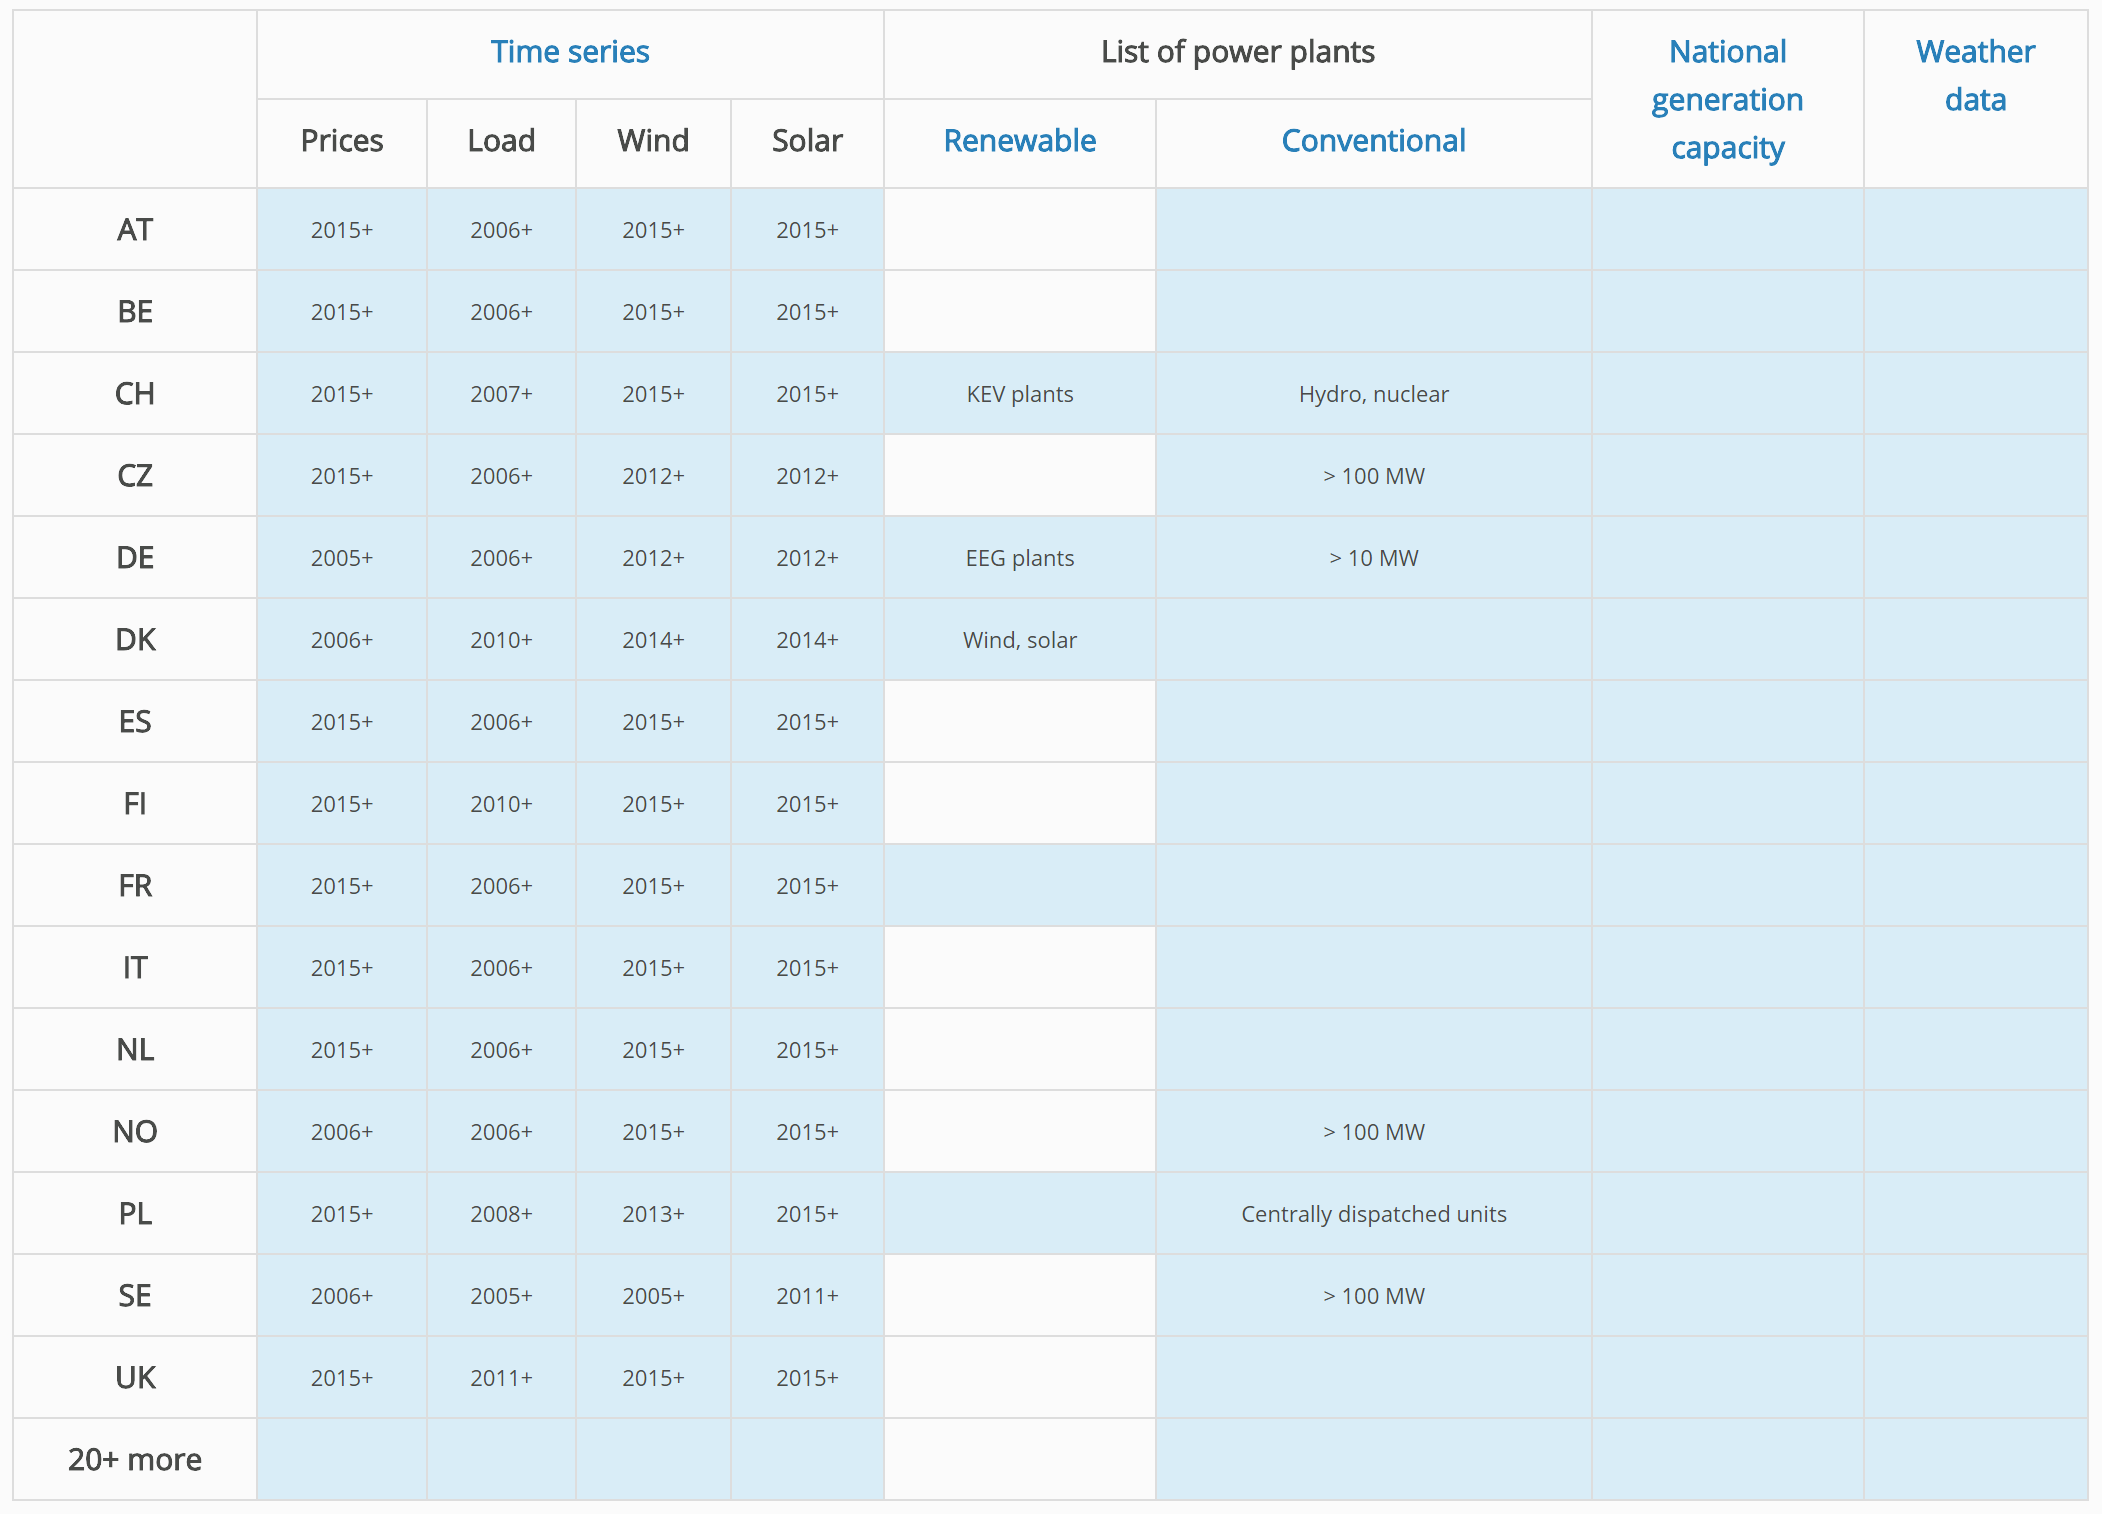
\includegraphics[width=1\textwidth]{figures/data_availability_overview.PNG}
    \caption{Overview of the current data availability}
    \label{fig:overview}
\end{figure}

Figure \ref{fig:energy_structure} displays the energy source structure we apply consistently to the first three packages.
\begin{figure}[!h]
    \centering
    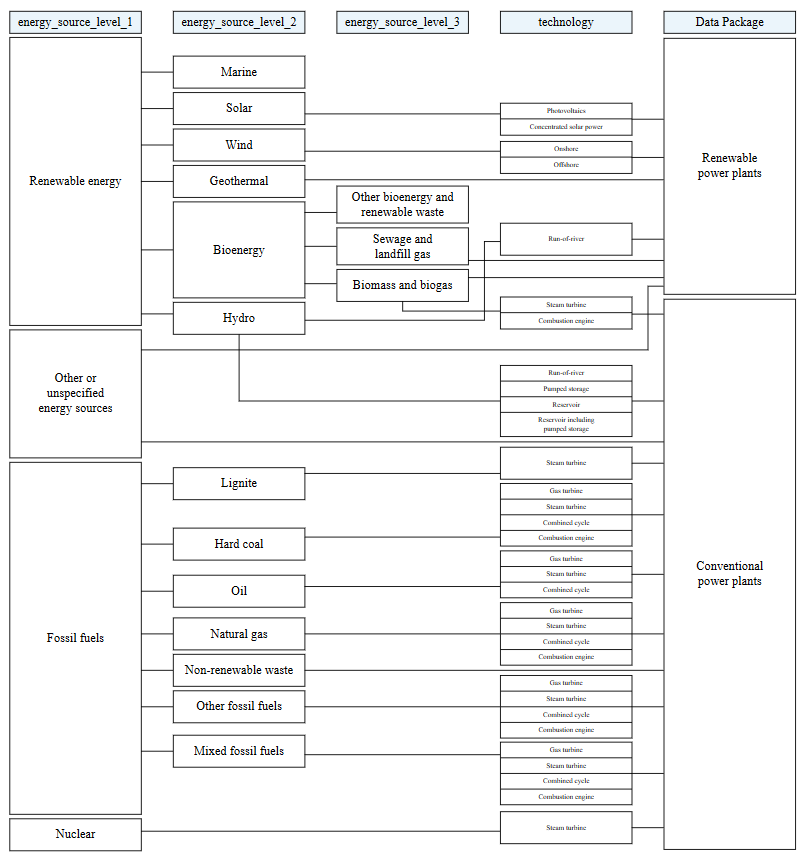
\includegraphics[width=1\textwidth]{figures/energy_source_tree.PNG}
    \caption{Classification}
    \label{fig:energy_structure}
\end{figure}

\subsection{Conventional power plants (Wolf)}
\paragraph{Content and Scope}
\paragraph{Geographic coverage}
\paragraph{Value added}

\subsection{National generation capacity (Wolf)}
\paragraph{Content and Scope}
\paragraph{Geographic coverage}
\paragraph{Value added}

\subsection{Renewable power plants (Frauke/Wolf-FL?)}
\paragraph{Content and Scope}
The renewable power plant data package contains a list of existing solar, wind, bio, run-of-river and geothermal power plants. Due to different data and parameter availability in the countries, one list is provided per country. These are of different accurancy and partly include different parameters. However, all state energy source and technology, electrical capacity (MW) and data source. If available in the data, the respective system operators (transmission and distribution), support schme ID or technology-specific parameters like hub height for wind turbines are included. While a high amount of parameters and units (more than 1.8 million power plant entries) are available for Germany, these only cover plants eligible under the renewable support scheme (EEG). Also for Switzerland just the supported plants are provided (Swiss feed in tariff KEV) since these are well documented and information is openly provided. For Denmark, detailed data on solar and wind power plants including rotor diameter etc. is provided, but no other technologies. Aggregated capacity per energy source and municipality is stated in the lists for Poland and France.

Most original data source either provide conventional or renewable power plants. However, especially with respect to hydro power, information overlaps and is difficult to correlate. With the objective to provide data packages that can be directly applied by the modellers, we tried to eliminate the overlap by clarifying which energy sources and which technologies are covered by the conventional and renewable data package as illustrated in \ref{fig:energy_structure}.

An additional output of this data package are the historic daily time series of the installed renewable capacities per energy source type for Germany. These are applied in the time series script: Since solar and wind feed-in time series are derived from real feed-in data, the absolute feed-in is rising during the year due to increasing installed capacity. For deriving the relative, normalized feed-in, the corresponding installed capacity is required.

\paragraph{Geographic coverage} Currently lists of German, Danish, Swiss, Polish and French renewable power plants are provided. Since the location of renewable power plants is decisive for resulting feed-in of wind and solar, the geographic location is provided where information was available. This is the case for Germany, Denmark and France. These coordinates are of different accurancy since they are partly derived from zip-codes or districts.


\paragraph{Value added}
The amount of renewable energy units exceed by far the conventional ones due to smaller unit size, which makes processing tedious and manual verification unit by unit verification impossible. Furthermore, naming conventions and classification of renewable energy technologies and sources differ significantly between countries. The added value of the script is thus bringing it to the same energy source structure as well as to the same formatting. Although some paramters differ between the country scripts, the country lists can be consistently combined for the cut set of essential parameters and directly applied for power system models. Furthermore, inconsistent data is marked and can thus easily be filtered out.

\subsection{Time series (Jonathan)}
\label{subsec:time series}

\paragraph{Content and Scope}
The time series data package contains highly granular time series data, including the following variables:
\begin{itemize}
    \item Power consumption (load)
    \item Power generation by varaiable renewables (wind and solar) and share of production capacity 
    \item Day-ahead power prices
\end{itemize}

\paragraph{Geographic coverage}
Overall, 35 countries are covered. coverage varies between variables, however and improves with time. While load data is published for all European countries, availability of renewable generation data varies between countries. While historic records of day-ahead prices could be purchased from power exchanges, they are freely available only since 2015, when the ENTSO-E Transparency Platform was introduced.

\paragraph{Value added}
While from 2015 onwards, many of the data are available from the ENTSO-E Transparency Platform, earlier records have to be obtained through individual national sources. Data are extracted mostly from national TSO's websites, ENTSO-E's "Monthly statistics data collection" as well as ENTSO-E Transparency. Data formats vary greatly depending on the source: Some TSOs allow downloading one file containing all available data (Amprion), while others require downloading and combining monthly (TenneT) or even daily files (PSE). Depending on the national market set-up, data have a resolution of either 15 (i.e. Austria, Germany and some neighbours), 30 (i.e. the British Isles) or 60 minutes (all other countries). The time series data package combines all data with the same temporal resolution in one file each, greatly fascilitating it's use for modellers. Additionally, 15 and 30 minute data are aggregated to 60 minutes in order to provide one file with maximal geographic coverage.

Power system modelling usually requires time series data to be complete for the period under consideration. Many time series however are missing data for periods ranging from a few hours to many months. Individual data are commonly missing during the daylight-savings time fall back in October. Within the time series data package, data gaps up to 2 hours are filled by applying linear interpolation. In these cases, tables are annotated with a marker, allowing users to trace back where interpolation has been applied. Longer periods of missing data are left as-is.

\subsection{Weather data (Frauke/Martin?)}

\paragraph{Content and Scope}
The weather data package provides a script to automatically download and process wind, solar and temperature data based on the MERRA-2 dataset (TODO REFERENZ) made available by NASA (illustration: Figure \ref{fig:weather data}). It differs significantly to the other data packages as no one click-download of the already processed data is available on the platform. Due to the size of the data which can reach GB and TB if a high amount of variables, a long timespan and a huge geographical area is chosen, the strategy here is to provide a documented methodological script and a data sample for the year 2016 for Germany. The user is thus enabled to receive a chosen set of parameters of a specified area and time span, by running the script on the own computer. Resulting data can be formatted either in csv or sql-format. Parameters covered are
\begin{itemize}
 \item wind velocity in 2, 10 and 50 meters height and roughness length
 \item solar radiation
 \item temperature
 \item air density and pressure
\end{itemize}

Since the total top-of the-atmosphere horizontal and the ground radiation in the original data is not what a energy modeller requires to calculate the resulting energy yield of a solar power plant, the script provides methods to transform these to direct/indirect radiation.

\begin{figure}[!h]
    \centering
    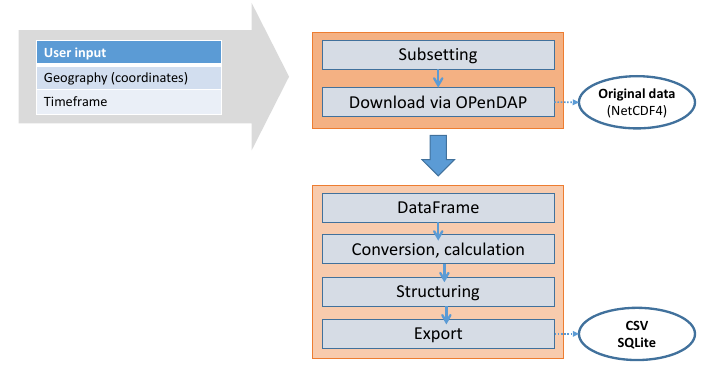
\includegraphics[width=1\textwidth]{figures/weather_data.png}
    \caption{Content and scope of the weather data script}
    \label{fig:weather data}
\end{figure}

\paragraph{Geographic coverage}
The reanalysis data has worldwide coverage in a resolution of 0.625 x 0.5. By specifying two coordinates in the script, a rectangular area can be chosen.

\paragraph{Value added}
Weather parameter for modelling are crucial due to the rising influence of wind and solar feed-in for the power system. The OPSD weather data script fills a gap between original meteorological data (e.g. MERRA-2) and ready-made feed-in time series. On the one hand direct usage of original datasets require knowlegde which one to choose of the hundreds of meteorological parameters and how to receive wind speed and solar radiation relevant for power-modelling. Additionally, the NetCDF-file format preferred by meteorologist due to its mutlidimensional option, is not directly compatible with data formats preferred by power system modellers and requires thus tedious processing. On the other hand, feed-in time series as provided in the data package described in \ref{subsec:time series} are less flexible for the automatic integration to own modelling code and restricted to the assumptions made for the calculation of the resulting electricity feed-in like e.g hub height of wind turbines. Thus, for power modellers who have the ambition of own feed-in calculations and require a long timespan of historic weather data, this script lowers the barrier of utilizing the wealth of available reanalysis weather data.
        
\section{Discussion and Outlook (Lion)}
\label{sec:discussion}
\begin{itemize}
    \item Wolf: hier insbesondere auf laufende Erweiterungen etc. eingehen, möglicherweise auch auf Zielgruppen etc. 
    \item Statistics on how the data is applied, how many users etc., maybe categorize the applications
    \item MaybesShow verification/validation results of bottom-up power plant data with national statisticsja
    \item The approach of OPSD is reproducible, flexible, possible to update and widely apply
    \item quality of the data, room for improvement: what specific?
    \item maintenance work is required
    \item Procedure cannot be applied for all data required for energy system modelling, e.g. for grid stuff probably, there database approaches are also required
    \item tools and knowledge for reproducible data processing and metadata storage is there but data education (documentation, organisation) for energy system modellers is a bottleneck while important
    \item legal issue is central, examples of improvement, but data knowledge and knowledge of open licences for original data owners is lacking
\end{itemize}

\section*{References}

\bibliography{mybibfile}

\end{document}